\documentclass[a4paper]{article}

\usepackage[a4paper,margin=2cm]{geometry}
\usepackage{amsmath}
\usepackage{graphicx}
\usepackage[table]{xcolor}
\usepackage{tikz}
\usepackage{minted}
\usepackage[clock]{ifsym}
\usepackage{subcaption} % subfigures
\usepackage{hyperref} % links in table of contents
\usepackage[strings]{underscore}

\usetikzlibrary{calc,positioning,shapes,arrows.meta,decorations.pathreplacing}
\graphicspath{ {./graphics/} }

\hypersetup{
	colorlinks,
	citecolor=black,
	filecolor=black,
	linkcolor=black,
	urlcolor=black
}
\numberwithin{figure}{section}
\numberwithin{table}{section}
\renewcommand{\arraystretch}{1.5}

\newcommand{\mi}{\mintinline}
\newcommand{\NA}{---}

\title{CS2031 - Assignment 2\\OpenFlow}
\date{2018-12-24}
\author{\url{https://git.nul.ie/dev/oof}\\\url{https://github.com/devplayer0/oof}\\Jack O'Sullivan\\\href{mailto:osullj19@tcd.ie}{osullj19@tcd.ie}}

\begin{document}
\maketitle
\tableofcontents
\pagenumbering{gobble}

\newpage
\pagenumbering{arabic}
\section{Introduction}
The goal of this assignment was to develop an implementation of an OpenFlow-like protocol for a controller and routers, as well routing some kind of traffic using the ``OpenFlow'' implementation.

\section{Implementation}
The implementation of the assignment is called ``Oof'' (a recursive acroynm: ``Oof: OpenFlow'').
\subsection{Design choices / features}
\begin{itemize}
	\item Rust was used again for this project for similar reasons to Assignment 1
	\item The controller implements Link-state routing (calculating shortest routes with Dijkstra's algorithm)
	\item Oof is able to (at least partially) replace the routing system built into the Linux kernel and route \textbf{real IPv4 traffic on real hardware}!
	\item The assignment was split into a number of subprojects:
		\begin{itemize}
			\item \mi{c}{oof-controller}: Oof controller implementation and binary
			\item \mi{c}{oof-router}: Oof router implementation and binary
			\item \mi{c}{oof-common}: Common code used by controller / router
		\end{itemize}
	\item The control plane protocol runs on top of TCP, greatly reducing its complexity
	\item A Wireshark dissector was again written for the protocol
	\item To aid testing, a few Python scripts were written to set up a virtual networking environment:
		\begin{itemize}
			\item \mi{c}{test_net.py} creates a ``virtual network'' from a YAML file using Linux network namespaces
			\item \mi{c}{start_infrastructure.py} reads the same YAML document and starts controller and router processes automatically
		\end{itemize}
\end{itemize}

\newpage
\subsection{Protocol} \label{sec:protocol}
The Oof control plane protocol is made up of 6 different message types. Each contains a 1-byte message type and (usually) some kind of payload. As with JQTT, all integers are represented in network / big endian. Since the protocol runs on top of TCP, the number of control messages is reduced.

\subsubsection{Wireshark dissector}
The Wireshark dissector once again utilises the Wireshark Lua API. It can be installed in the same way as the JQTT dissector. When enabled, Oof messages will be decoded:

\begin{figure}[h!]
	\centering
	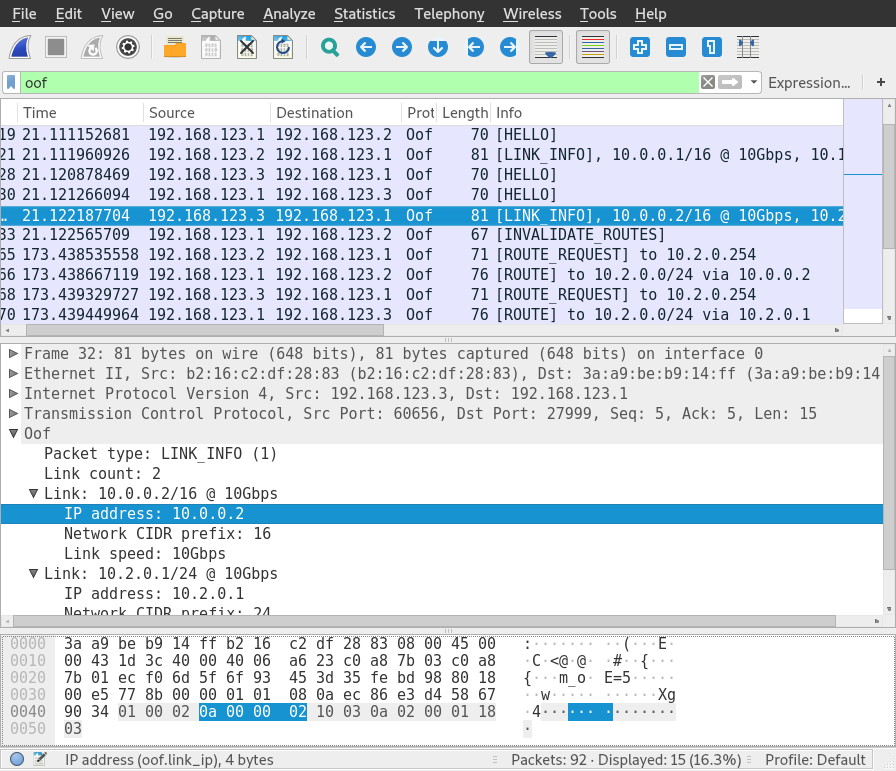
\includegraphics[width=\textwidth]{dissector}
	\caption{Oof messages decoded in Wireshark}
	\label{fig:dissector}
\end{figure}

Figure~\ref{fig:dissector} shows Oof messages decoded from TCP segments with detailed output, similarly to the JQTT version. Filtering, the detail tree and info column work in the same manner as before. Note the dissector will produce a distinct entry in the Wireshark list for each message, re-assembling / splitting TCP segments as necessary.

\newpage
\subsection{Packet types}
As explained in section~\ref{sec:protocol}, there are 6 distinct message types in Oof. The structure and purpose of each is explained in detail in this section (in order of the type number which takes up the first byte of each message).

\subsubsection{\mi{c}{HELLO}}
\mi{c}{HELLO} is a very a simple message sent by both the controller and routers once a TCP connection has been established. After the packet type byte, the magic sequence ``Oof'' appears (ASCII representation). Once connected to the controller, a router will send this message. The controller will send its own \mi{c}{HELLO} in response.

\subsubsection{\mi{c}{LINK_INFO}}
This message is sent by a router to the controller to inform a router of the links it has. The controller will then update its routing tables accordingly. \mi{c}{LINK_INFO} can be sent at any time, but is always sent at router startup.

Structurally, this message is an array of ``link objects''. After the packet type byte, a 16-bit unsigned integer counts the number of links in the message. What follows is the actual link information, one set after another (no separation since each is a fixed length):
\begin{enumerate}
	\item Network card's IP address (stored as a 32-bit unsigned integer)
	\item Assigned IP CIDR prefix (stored as an 8-bit unsigned integer with a maximum value of 32)
	\item Link speed, stored as an 8-bit unsigned integer representing the possible values for an enum:
		\begin{itemize}
			\item \mi{c}{0}: ``Slow ethernet'' (10Mbps)
			\item \mi{c}{1}: ``Fast ethernet'' (100Mbps)
			\item \mi{c}{2}: Gigabit (1000Mbps)
			\item \mi{c}{3}: 10 Gigabit (10000Mbps)
			\item \mi{c}{4}: 40 Gigabit (40000Mbps)
			\item \mi{c}{5}: 100 Gigabit (100000Mbps)
		\end{itemize}
\end{enumerate}

\subsubsection{\mi{c}{ROUTE_REQUEST}}
\mi{c}{ROUTE_REQUEST} is sent by a router to the controller when it receives a packet which it doesn't know how to route (no entry in its local cached routing table).

Its structure is very simple: after the packet type, the destination IP (for which a route is required) is represented as a 32-bit unsigned integer.

\subsubsection{\mi{c}{ROUTE}}
A \mi{c}{ROUTE} message is sent by the controller to a router in response to a \mi{c}{ROUTE_REQUEST} upon successful lookup of a suitable route to the destination.

Essentially a ``route'' looks like the output when executing \mi{c}{ip route show} on Linux: the message consists of a CIDR network (which the destination IP from the \mi{c}{ROUTE_REQUEST} belongs to) and a next hop (which is reachable directly over one of the router's links).

The message's structure follows the order described above (IP addresses and the CIDR prefix are represnted in the same way as \mi{c}{LINK_INFO}:
\begin{enumerate}
	\item Network address (e.g. if the destination was 172.16.0.123, the network address would be 172.16.0.0)
	\item Network CIDR Prefix
	\item Next hop IP address
\end{enumerate}

\subsubsection{\mi{c}{NO_ROUTE}}
The controller will send this message to a router if it is unable to find a suitable route to the requested destination. The IP address for which a route was originally requested is provided so the router knows which \mi{c}{ROUTE_REQUEST} failed - the router will usually maintain a local cache of which destinations have no route.

Structurally this packet is identical to \mi{c}{ROUTE_REQUEST} except for the differing packet type.

\subsubsection{\mi{c}{INVALIDATE_ROUTES}}
\mi{c}{INVALIDATE_ROUTES} is sent by the controller to a router when the routing table has changed (for instance if a new router has connected to the controller with new links). It signals to routers that they should clear their locally cached routes (including the list of unroutable addresses).

\mi{c}{INVALIDATE_ROUTES} carries no information and only contains the packet type byte.

\subsection{Code structure}
As with the Flow control assignment, Oof is divided into crates, although here there are only three. There are also the two Python scripts and YAML description of a sample test network.

\subsubsection{Common code (\mi{c}{oof-common})}
This crate contains code shared by the controller and router crates. Essentially this just consists of a few utilities used by both:
\begin{itemize}
	\item A \mi{rust}{MessageType} enum
	\item Functions to send / await \mi{c}{HELLO} messages
	\item \mi{rust}{LinkSpeed} enum to parse and display link speed
	\item Other small utilities
\end{itemize}

\subsubsection{Controller}
The \mi{c}{oof-controller} crate contains the implementation of the Oof controller (including a command line executable).

The primary struct, \mi{rust}{Controller}, has a \mi{rust}{bind()} function which creates the primary TCP socket on the specified interface which listens on its own thread. When a new connection is opened, the controller will create a new \mi{rust}{Client} struct instance to handle it.

\mi{rust}{Controller} also holds a \mi{rust}{Network}, which represents the network and routing tables. \mi{rust}{Controller::net_as_dot()} calls into the \mi{rust}{Network} to produce a Graphviz DOT representation of the network (as a \mi{rust}{String}).

When a new \mi{rust}{Client} is created, it starts a new thread and waits for a \mi{c}{HELLO} message before entering a message processing loop. \mi{rust}{ClientInner} contains the relevant code to encode / decode the protocol as well as handle incoming messages.

\medskip
\noindent \mi{rust}{Network} represents the network as an undirected graph (provided by the \mi{c}{petgraph} crate), where the nodes are either routers \textbf{\underline{or}} networks and the edges are links. An example network looks like this:

\begin{figure}[h!]
	\centering
	\resizebox{\columnwidth}{!}{
		
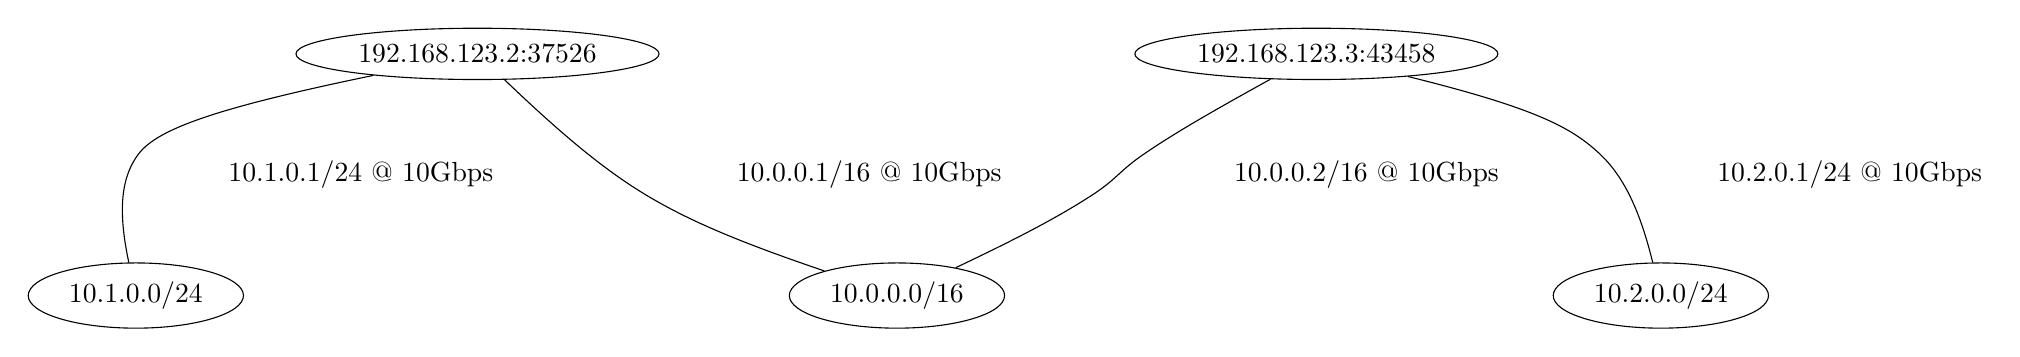
\begin{tikzpicture}[>=latex,line join=bevel,]
%%
\node (1) at (63.694bp,18.0bp) [draw,ellipse] {10.1.0.0/24};
  \node (0) at (186.69bp,105.0bp) [draw,ellipse] {192.168.123.2:37526};
  \node (3) at (488.69bp,105.0bp) [draw,ellipse] {192.168.123.3:43458};
  \node (2) at (337.69bp,18.0bp) [draw,ellipse] {10.0.0.0/16};
  \node (4) at (612.69bp,18.0bp) [draw,ellipse] {10.2.0.0/24};
  \draw [] (0) ..controls (92.281bp,85.488bp) and (71.526bp,77.954bp)  .. (64.694bp,69.0bp) .. controls (57.711bp,59.847bp) and (57.562bp,46.839bp)  .. (1);
  \definecolor{strokecol}{rgb}{0.0,0.0,0.0};
  \pgfsetstrokecolor{strokecol}
  \draw (144.69bp,61.5bp) node {10.1.0.1/24 @ 10Gbps};
  \draw [] (0) ..controls (216.56bp,76.41bp) and (232.17bp,63.273bp)  .. (247.69bp,54.0bp) .. controls (262.58bp,45.112bp) and (280.05bp,37.548bp)  .. (2);
  \draw (327.69bp,61.5bp) node {10.0.0.1/16 @ 10Gbps};
  \draw [] (3) ..controls (447.07bp,82.04bp) and (436.27bp,75.509bp)  .. (426.69bp,69.0bp) .. controls (417.8bp,62.95bp) and (416.74bp,59.821bp)  .. (407.69bp,54.0bp) .. controls (396.09bp,46.533bp) and (382.74bp,39.354bp)  .. (2);
  \draw (506.69bp,61.5bp) node {10.0.0.2/16 @ 10Gbps};
  \draw [] (3) ..controls (567.91bp,85.402bp) and (580.61bp,78.423bp)  .. (590.69bp,69.0bp) .. controls (600.0bp,60.311bp) and (605.55bp,47.023bp)  .. (4);
  \draw (680.69bp,61.5bp) node {10.2.0.1/24 @ 10Gbps};
%
\end{tikzpicture}


	}
	\caption{Example network (Graphviz created via \mi{rust}{Network::as_dot()})}
	\label{fig:test-net}
\end{figure}

The network shown in Figure~\ref{fig:test-net} is the one described in the provided \mi{c}{test_net.yaml}. It shows two routers (192.168.123.2 and 192.168.123.3) and three networks (10.1.0.0/24, 10.0.0.0/16 and 10.2.0.0/24) along with the links each router has to each network (showing the IP of the network card and the link speed).

When \mi{rust}{Network::update_router_links()} is called when a new router appears with its links, the \mi{rust}{Router} struct will add itself as a node to the graph, add nodes for each network it has a link to (if they don't already exist) and create edges representing its links to those networks. \mi{rust}{Router::calculate_routes()} will then be called for every router to create routing tables.

The first portion of this function is an implementation of Dijkstra's algorithm (using a priority queue to store the unvisited nodes with cost calculated as $\frac{speed_{iface}}{1000}$). After this, a routing table for every network is produced by walking backwards through the resulting ``node / cost / previous'' triple list (with network nodes filtered out) until the router's node is found.

The node just before the router building the table will always be the network through which the next hop is reachable and the node before that will be the router representing the next hop. The next hop retrieved by looking up the router in a hashtable using its control plane address (the second last node stores this) and reading the address of the link into the network through which it is reachable.

\subsubsection{Router}
\mi{c}{oof-router} provides a router binary and implements the control plane client and actual packet routing.

\mi{c}{client.rs} provides \mi{rust}{Router}, a struct analagous to \mi{rust}{Client} in \mi{c}{oof-controler} which connects to the controller and handles incoming messages in a new thread. \mi{rust}{RouterInner} encodes / decodes packets similarly to how \mi{rust}{ClientInner} does.

\mi{rust}{Router::update_links()} calls into \mi{rust}{RouterInner} to send a \mi{c}{LINK_INFO} message to the controller.

\mi{rust}{Router::find_route()} will check the local routing cache for either an existing route or return immediately if the requested IP address is in the unroutable addresses list. If there are no entries in the cache, a \mi{c}{ROUTE_REQUEST} will be sent to the controller and the function will block until there is either a \mi{c}{ROUTE} or \mi{c}{NO_ROUTE} response (utilising \mi{rust}{std::mpsc} for synchronisation).

\medskip
\noindent Actual routing is performed by the \mi{rust}{RawRouter} struct. It creates a \mi{rust}{Router} instance to handle the control plane, gathers information about available network interfaces on the system and begins routing traffic on a new thread.

\mi{rust}{RawRouterInner::new()} establishes the list of links from network interfaces on the system, as long as each:
\begin{itemize}
	\item Is not loopback interfaces
	\item Is up
	\item Is not on the list of user-provided interfaces to be ignored
	\item Has an IPv4 address
	\item Is not the interface on which the connection to the controller has been established
\end{itemize}

\mi{rust}{Router::update_links()} will then be called with the first IPv4 address (and CIDR prefix) on each interface (and their link speeds obtained from \mi{c}{/sys/class/net/<interface>/speed}).

\mi{rust}{RawRouter} makes extensive use of the \mi{rust}{pnet} crate (or rather a fork maintained at \url{https://github.com/devplayer0/libpnet} which allows access to the file descriptor of sockets so they can be \mi{c}{poll()}'d) for encoding / decoding various network protocols.

A packet socket will be opened on each interface (using \mi{rust}{pnet}) and \mi{rust}{RawRouterInner::read_and_process()} will run in a loop, blocking until an Ethernet frame arrives from one or more interfaces. Note that since packet sockets are essentially the kernel providing a \textbf{copy} of Ethernet frames, the on-link routes generated automatically when an address is added to an interface are deleted (if they exist) to prevent the kernel from doing any kind of processing of its own.

\mi{rust}{RawRouterInner::handle_packet()} will then be called to perform an appropriate action:
\begin{itemize}
	\item If the EtherType of the frame is an ARP packet (the only EtherType handled is IPv4) and the parsed ARP packet is a request for the address of the interface on which the packet arrived, a reply will be sent with the interface's MAC (with the on-link route removed the kernel will not respond to ARP requests)
	\item If the IPv4 TTL of the packet is zero, it will be dropped as invalid
	\item If upon decreasing the TTL by 1, the TTL has reached 0, the packet will be dropped and an ICMP Time Exceed packet will be sent to the sender (this is implemented mainly to facilitate use of the \mi{c}{traceroute} command)
	\item If the packet is an ICMP Echo Request for one of the router's interfaces, an ICMP Echo Response will be sent
	\item Otherwise, \mi{rust}{Router::find_route()} will be called to find where the packet should go next
		\begin{itemize}
			\item If a suitable route is not found, an ICMP Destination Unreachable packet (with the ICMP code set to ``Destination Network Unknown'') will be sent
			\item Otherwise, the IPv4 header checksum will be re-calculated (since the TTL has changed) and the packet will be sent to the next hop (the source and destination MAC addresses will be updated accordingly, with an ARP lookup being performed if necessary)
		\end{itemize}
\end{itemize}

Sending ICMP packets is fairly explanatory, once the IPv4 packet has been constructed, the packet is sent to its destination as if it was another packet to be forwarded (i.e. an ARP lookup may need to be performed).

ARP lookups involve constructing the ARP request, sending it to the broadcast address and blocking for up to 500ms until a valid reply is received. It will then be inserted into a local ARP table. Other packets will be pushed to the back of a queue which will be drained and handled on the next execution of \mi{rust}{RawRouter::read_and_process()} before polling the packet sockets.

\subsubsection{Test network setup script (\mi{c}{test_net.py})}
The YAML file read by this script (and \mi{c}{start_infrastructure.py}) contains the following:
\begin{itemize}
	\item A table of networks mapped by name to CIDR network
	\item A list of ``nodes'' (mapped by name), each of which contains:
		\begin{itemize}
			\item A list of networks mapped by name (as defined above) to an optional IP address
			\item An optional set of routes (mapped by network to next hop)
		\end{itemize}
\end{itemize}

After parsing this document, the following steps will be followed (utilising the \mi{python}{pyroute2} library, a pure Python binding to \mi{c}{NETLINK} to manage namespaces and interfaces):
\begin{enumerate}
	\item A Linux network bridge will be created in the host namespace for each network which acts as a switch (to which each node will be connected).
	\item A network namespace will be created for each node, and then:
		\begin{enumerate}
			\item Its loopback interface will be put up
			\item A \mi{c}{veth} pair will be created for each network to which this node should be connected to. One ``end'' of this virtual ``network cable'' will be attached to the appropriate bridge in the host namespace and the other will be assigned either the specified IP address from the YAML document or the next available IP address in the network.
			\item Any routes listed for this node in the YAML will be created (including a potential default route)
		\end{enumerate}
\end{enumerate}

Once the setup is completed, the script will block until it receives \mi{c}{SIGINT} or \mi{c}{SIGTERM}. At this point, all of the namespaces will be deleted (effectively destroying all of the \mi{c}{veth} pairs) along with the bridges on the host.

\medskip
\noindent Note that the namespaces will not be removed by the kernel until all processes running in them have stopped.

\subsubsection{Test network ``infrastructure'' script (\mi{c}{start_infrastructure.py})}
This script is relatively simple and reads optional \mi{c}{is_controller} and \mi{c}{is_router} flags added to the YAML document for each node, executing the corresponding binary in the appropriate namespace using \mi{c}{ip netns exec <command>} (using \mi{c}{pyroute2}'s \mi{python}{NSPopen()} causes issues since the \mi{c}{sysfs} presented to the process will be the host's, meaning \mi{bash}{/sys/class/net/*} will contain the host's interfaces).

It will pipe the output of the executed processes (with each line prepended by its node name to tell them apart) to its own \mi{c}{STDOUT}, blocking like \mi{c}{test_net.py} until \mi{c}{SIGINT} / \mi{c}{SIGTERM} is received. \mi{c}{SIGTERM} will then be sent to each process.

\section{Testing and performance}
\subsection{Using the virtual network scripts}
The testing process is made relatively easy using \mi{c}{test_net.py} and \mi{c}{start_infrastructure.py} with the provided \mi{c}{test_net.yaml}. However, there are a few things which should be noted:
\begin{itemize}
	\item \mi{c}{iptables} rules (including those created by Docker) may cause issues
	\item IP forwarding (\mi{bash}{sysctl -w net.ipv4.ip_forward=1}) is not needed (Oof replaces this!)
	\item \textbf{Checksum and TCP / UDP segment offload may cause difficult to locate issues.} Likely due to the fact there is no hardware to offload these tasks to (meaning this work may be done somewhere in the kernel at the network layer instead of at the link layer where a real network card operates), TCP / UDP checksums will not be calculated correctly and very large (bigger than MTU) TCP segments will be delivered to the packet sockets which are then impssible to transmit. To work around this problem, run \mi{bash}{ethtool -K <interface name> tx off} for the interfaces being used at either end of communication (e.g. on the outgoing interface for a client node and the corresponding interface on a server node). This is not \textit{not} necessary for router nodes.
\end{itemize}

\subsubsection{Performance}
Commands run to perform this test:
\begin{itemize}
	\item \mi{bash}{ip netns exec server_2 iperf -s}
	\item \mi{bash}{ip netns exec server_1 iperf -c 10.2.0.254}
\end{itemize}

This results in routing traffic from \mi{c}{server_1} (which has a normal Linux routing setup) through \mi{c}{router_a} and \mi{c}{router_b} to \mi{c}{server_2} (which also uses plain Linux routing). Utilising release builds on a Dell XPS 13 9370 (with a quad-core Intel Core i7-8550U), \mi{c}{iperf} reported 907Mbps throughput.

\subsection{On real hardware}
For this test, a Raspberry Pi 2 and Raspberry Pi 3 were used as routers (i.e. running \mi{c}{oof-router}). The network is similar to that of \mi{c}{test_net.yaml}:
\begin{itemize}
	\item A workstation with a 16-core AMD Threadripper 1950X clocked at 4.0GHz fills the role of \mi{c}{server_2} (and the controller)
	\item The Dell XPS 13 9370 described in the previous section is used as \mi{c}{server_1}
	\item The Raspberry Pi 3 is \mi{c}{router_a}
	\item \mi{c}{router_b} is the Raspberry Pi 2
\end{itemize}

The CIDR networks are the same, with the exception of the control network, which is \mi{c}{172.16.0.0/24} instead of \mi{c}{192.168.123.0/24}.

\subsubsection{Physical configuration}
\begin{figure}[h!]
	\centering
	\includegraphics[width=\textwidth]{hardware-overview}
	\caption{Test hardware overview}
	\label{fig:hardware-overview}
\end{figure}

Figure~\ref{fig:hardware-overview} all four pieces of hardware connected together. From top to bottom, the photo shows \mi{c}{server_2} / controller, \mi{c}{server_1}, \mi{c}{router_b} and \mi{c}{router_a}. A few things to note:
\begin{itemize}
	\item The control plane actually runs over the primary home LAN. The Raspberry Pis and laptop are connected over WiFi (a Ubiquiti UniFi AP AC Pro, the Raspberry Pi 2 has no built-in WiFi so is using a USB dongle) and the desktop is connected directly to the main router via a 10Gb fibre link.
	\item Although a managed network switch is present, it is \textbf{only used for its VLAN functionality} - due to a shortage of USB network cards, \mi{c}{router_a} is connected to \mi{c}{server_1} through one VLAN and to \mi{c}{router_b} through another.
\end{itemize}

\subsubsection{Performance}
\begin{figure}[h!]
	\centering
	\includegraphics[width=\textwidth]{hardware-results}
	\caption{Test hardware results}
	\label{fig:hardware-results}
\end{figure}

Running the same commands as in the virtual environment test (resulting in traffic routing through the 2 Raspberry Pis), \mi{c}{iperf} reported 57Mbps (compared to 87Mbps using kernel routing on in place of Oof on the Raspberry Pis), again using release builds. \mi{c}{oof-router} was cross-compiled on the workstation for the \mi{c}{aarch64-unknown-linux-gnu} and \mi{c}{armv7-unknown-linux-gnueabihf} targets respectively to run on the Pis.

It is worth noting that the Raspberry Pis have relatively low performance hardware to start. The Raspberry Pi 2 is powered by a quad-core Cortex-A7 (32-bit ARMv7 clocked at 900MHz) and the Raspberry Pi 3 has a quad-core Cortex-A53 (64-bit ARMv8 clocked at 1.4GHz). The onboard network interfaces are also limited to 100Mbps and are connected internally over USB.

\newpage
\section{Reflection / limitations}
Overall, a reasonable implementation of an OpenFlow-like protocol (made more interesting by routing real traffic) was created in Oof. As with the first assignment, there are some limitations:
\begin{itemize}
	\item IPv6 is completely unsupported. The protocol, control plane implementation and routing system would need to be significantly reworked for this.
	\item Userspace routing will always result in relatively poor performance due to the need for several copies of packets to be made, as well as frequent context switching
	\item If a link goes down / up, it will not be handled. \mi{c}{oof-router} would probably crash. It would need to be re-worked to handle these events gracefully and inform the controller.
	\item There are no rules to decide how packets should be routed besides which route is the shortest and has more bandwidth. More advanced rules (including those based on Layer 4 or possibly even Layer 7 DPI) would be desirable, but would again require a major rework of all components in the system.
\end{itemize}

\end{document}
# vim: nofoldenable
